\section{Introduction}
\label{sec:intro}

Modern machine learning services are increasingly deployed as distributed
microservice systems~\citep{qiu2020firm,alibabatrace2022}. A single user
request may pass through many interacting components: frontend services,
retrieval services, ranking services, payment or logging services,
caches, databases, and model serving endpoints. Keeping such systems
reliable requires continuous resource allocation. Too few replicas lead
to latency spikes and service-level violations; too many replicas waste
compute. Autoscaling is therefore a core control problem for distributed
machine learning services: decide where to add or remove capacity, under
changing demand, while balancing latency, reliability, and cost.

Production autoscaling, however, remains largely reactive. Standard
controllers such as the Kubernetes Horizontal Pod Autoscaler
\citep{rzadca2020autopilot,googlecloud2025hpa,aws2025hpa} scale only
after utilization or latency signals indicate that the system is already
under pressure. Recent extensions augment HPA with short-horizon
forecasting or adaptive thresholds
\citep{pozdniakova2024sla,mondal2023predictive,ahmad2024smarthpa,santos2024gwydion},
yet still trigger scaling rules from a forecast metric rather than from
a simulated future trajectory. Safer deployments often compensate by
keeping extra replicas alive at all times. This creates a familiar but unsatisfactory trade-off: reactive
scaling is cheap but late, while static over-allocation is safer but
expensive. The problem is not only that existing controllers use simple
thresholds. More fundamentally, they act without a learned model of
the system: they do not know how a scaling action will propagate
through the service graph, how it will change downstream load and
latency, or whether it will create a future service-level violation.

We will refer to this missing capability as \emph{imagination}: the
ability of an autoscaler to ask counterfactual questions before acting,
in the spirit of learned world models that have proven effective for
planning in other domains~\citep{ha2018worldmodels,hafner2025dreamerv3}.
If we add replicas to the frontend, will the bottleneck move to checkout? If we scale the
recommendation service, will latency improve or will traffic shift to
the product catalog service? If we reduce capacity now, will the system
remain safe over the next few control steps? Current autoscalers mostly
act, observe, and correct. They do not simulate the consequences of their
actions before those actions reach the real cluster.

\begin{figure*}[t]
\centering
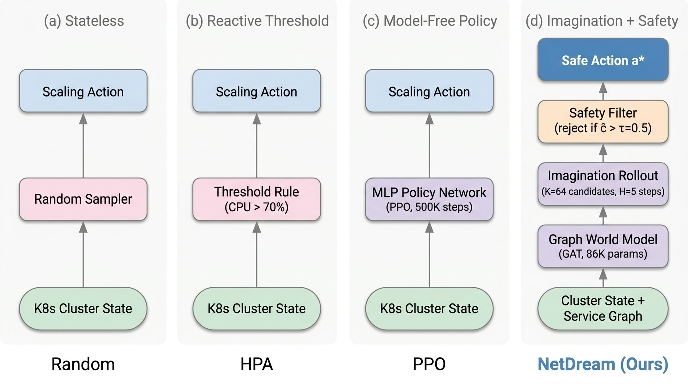
\includegraphics[width=\textwidth]{figures/fig_motivation.pdf}
\caption{\textbf{Why NetDream.}
Existing Kubernetes autoscalers map the current cluster state directly
to a scaling action: \textbf{(a)}~Random samples uniformly,
\textbf{(b)}~HPA reacts when CPU crosses a threshold, and
\textbf{(c)}~PPO learns a model-free policy. None of them imagine
future states before acting. \textbf{(d)}~NetDream inserts a graph
world model and a safety filter into this loop, so that candidate
scaling actions are first rolled out in imagination, scored, and
rejected if they are predicted to violate service-level constraints.}
\label{fig:motivation}
\end{figure*}

To answer the above questions and fill the research gap, we present
NetDream, a graph world model for safe autoscaling of distributed
machine learning services. NetDream represents a microservice
application as a graph, where nodes are services and edges are
service-call dependencies. While prior work has applied graph neural
networks to predict tail latency~\citep{park2021graf} or to learn
model-free actor--critic policies for autoscaling~\citep{chen2025graphpilot},
and digital-twin approaches~\citep{karma2025} have built unstructured
neural transition models of clusters, NetDream is, to our knowledge, the
first to combine a graph-structured dynamics model with imagination-based
planning and an explicit safety filter. It learns action-conditioned dynamics over
this graph: given the current service states and a candidate scaling
action, the model predicts how load, latency, replicas, reward, and
violation risk will evolve. At runtime, NetDream uses this learned model
inside an imagination-based planner. The planner rolls out multiple
future scaling trajectories, rejects those predicted to violate
service-level constraints, and executes only the first action of the best
safe plan. In this way, NetDream turns autoscaling from threshold-based
reaction into topology-aware planning over a learned model of the
system.

This formulation is operationally practical.
NetDream does not require an online reinforcement-learning agent to
explore risky actions in the real cluster~\citep{qiu2023aware,zhang2025kiss}.
Instead, it learns from logged transitions and uses the learned world
model as a simulator for planning.
The safety mechanism is also explicit: candidate futures whose predicted
violation risk exceeds a threshold are filtered out before execution.
This makes the controller closer to how human operators reason about
infrastructure: compare possible actions, reject unsafe ones, and choose
the lowest-cost safe plan.

\begin{figure*}[t]
\centering
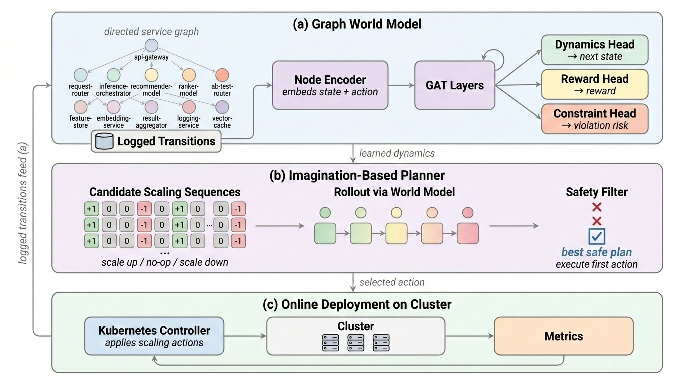
\includegraphics[width=\textwidth]{figures/fig_overview.pdf}
\caption{\textbf{NetDream for safe autoscaling of distributed machine
learning services.}
NetDream learns a graph world model of a microservice application
(illustrated here on a representative ML serving graph: api-gateway,
inference-orchestrator, recommender / ranker / embedding services,
feature store, etc.). Given the current service states and candidate
scaling actions, the model predicts future state changes, reward, and
service-level violation risk. A planning module rolls out multiple
candidate action sequences in imagination, rejects unsafe futures
through a learned safety filter, and executes the first action of the
best safe plan. Our empirical evaluation (Section~\ref{sec:experiments})
follows the standard Kubernetes autoscaling benchmarking practice and
uses Google's Online Boutique~\citep{googlecloud2023onlineboutique} —
the 11-service / 14-edge testbed adopted by recent GNN-based autoscaling
work~\citep{park2021graf,meng2023deepscaler,chen2025graphpilot} —
as a topologically equivalent representative of this microservice
class.}
\label{fig:overview}
\end{figure*}

We evaluate NetDream on a production-grade AWS Kubernetes deployment of
Online Boutique~\citep{googlecloud2023onlineboutique}, an 11-service,
14-edge microservice graph with a 66-dimensional system state and
48,000 collected transitions. The autoscaler is stress-tested under
four workload regimes (steady traffic, variable demand, bursty spikes,
and flash crowds) generated with Locust~\citep{locust} and replayed
from production microservice traces~\citep{alibabatrace2022}. We compare against
standard reactive autoscaling, static over-provisioning strategies,
random scaling, model-free reinforcement learning, and an ablation of
NetDream without the safety filter.

Our results show that graph-world-model planning is a more cost-efficient
path to safe autoscaling than reactive control or static
over-provisioning. NetDream-Safe sits on the cost--safety Pareto frontier
on a real AWS EKS deployment, and removing graph structure degrades
one-step prediction by $11\times$. We defer the per-workload numbers
and ablations to Section~\ref{sec:experiments}, and provide cross-domain
validation (power grid, water network, epidemic mobility graph) as
supplementary evidence that the architecture is not Kubernetes-specific
in Appendix~\ref{app:generalizability}.

Overall, this paper makes three contributions:

\begin{itemize}
\item We formulate autoscaling for distributed machine learning services
as planning with a learned graph world model. Instead of reacting to
threshold crossings, NetDream predicts the multi-step consequences of
scaling actions across the service graph before execution.

\item We introduce an imagination-based safety filter for autoscaling.
The planner rolls out candidate scaling sequences inside the learned
world model and rejects plans predicted to cause future service-level
violations.

\item We demonstrate cost-efficient safe autoscaling on a real AWS
Kubernetes deployment. On the Online Boutique benchmark, NetDream
achieves substantially better cost--safety trade-offs than reactive
autoscaling, static over-provisioning, model-free reinforcement learning,
and unsafe planning ablations.
\end{itemize}